\documentclass[tikz,border=3.14mm]{standalone}
\usepackage{tikz}

\begin{document}
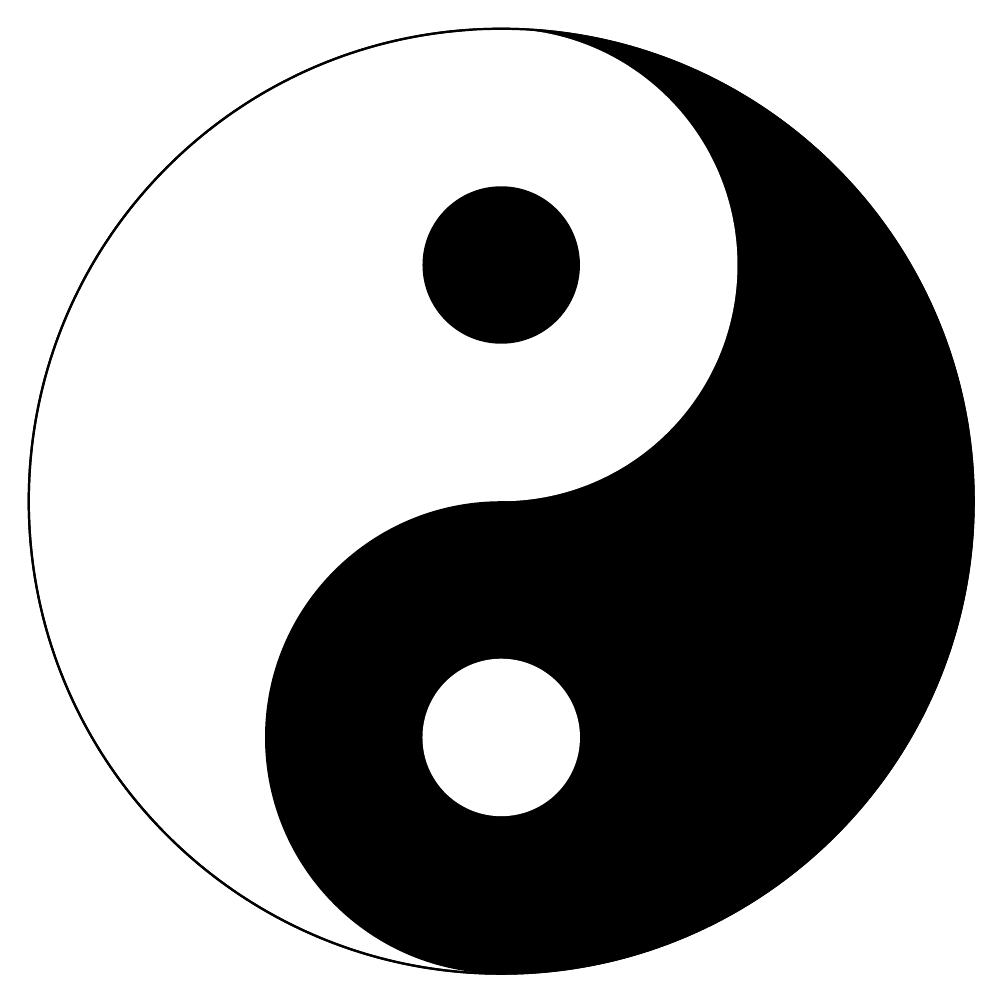
\begin{tikzpicture}

% 绘制阴阳鱼的大圆
\filldraw[thick, fill=white] (0,0) circle(6);

% 绘制黑色部分(右半圆涂黑)
\fill[black] (90:6) arc(90:-90:6) -- cycle;

% 绘制鱼头鱼尾
% 黑色半圆中画大圆半径1/2的白色实心圆
\fill [white] (90:3) circle(3);
% 白色半圆中画大圆半径1/2的黑色实心圆
\fill [black] (-90:3) circle(3);

% 绘制鱼眼
% 白色半圆中画大圆半径1/6的白色实心圆
\fill [black] (90:3) circle(1);
% 白色半圆中画大圆半径1/6的黑色实心圆
\fill [white] (-90:3) circle(1);

\draw[thick] (0,0) circle(6);

\end{tikzpicture}
\end{document}